
\section{Existing ontology work}
\label{existingontologies}

One of the key aspects of FAIR ontologies is the active reusability of existing
ontologies.

\subsection{The Open Energy Ontology}

The OEO has been in active development since 2021 with several releases since
then. It exists to address a technical gap associated with knowledge management
in the field of energy systems analysis. Said gap is the lack of common
semantics to annotate and share datasets and tools associated with the
mentioned discipline. The ontology is part of a larger data ecosystem called
the Open Energy Family (OEF), which allows researchers to share data sources
and results in accordance with the FAIR principles. It has had moderate
success, particularly within the context of projects associated to the OEF such
as the Open Energy Platform (OEP) \cite{Hulk.2024}. One of the characteristics
that makes this and other FAIR ontologies transparent and accessible is the
fact that it is being openly developed in a shared
repository\footnote{https://github.com/OpenEnergyPlatform/ontology}. An
important work on the inclusion of concepts coming from the transport sector
was performed by \cite{Mittermeier.2023}, who did several implementations
associated to the topic. However since the size of the task is larger than what
can be achieved during a master thesis, many implementations were left open in
the form of Github Issues. In some of these issues it was made clear that the
scope of the OEO is in some cases beyond what is often necessary to represent
phenomena in the transport sector. During the rest of this section we will
proceed to describe what is already in the ontology that is relevant to our
subject, what kind of discussion has been done and


\begin{figure}[h]
    \caption{Open energy ontology electric vehicle commitments.}
    \centering
    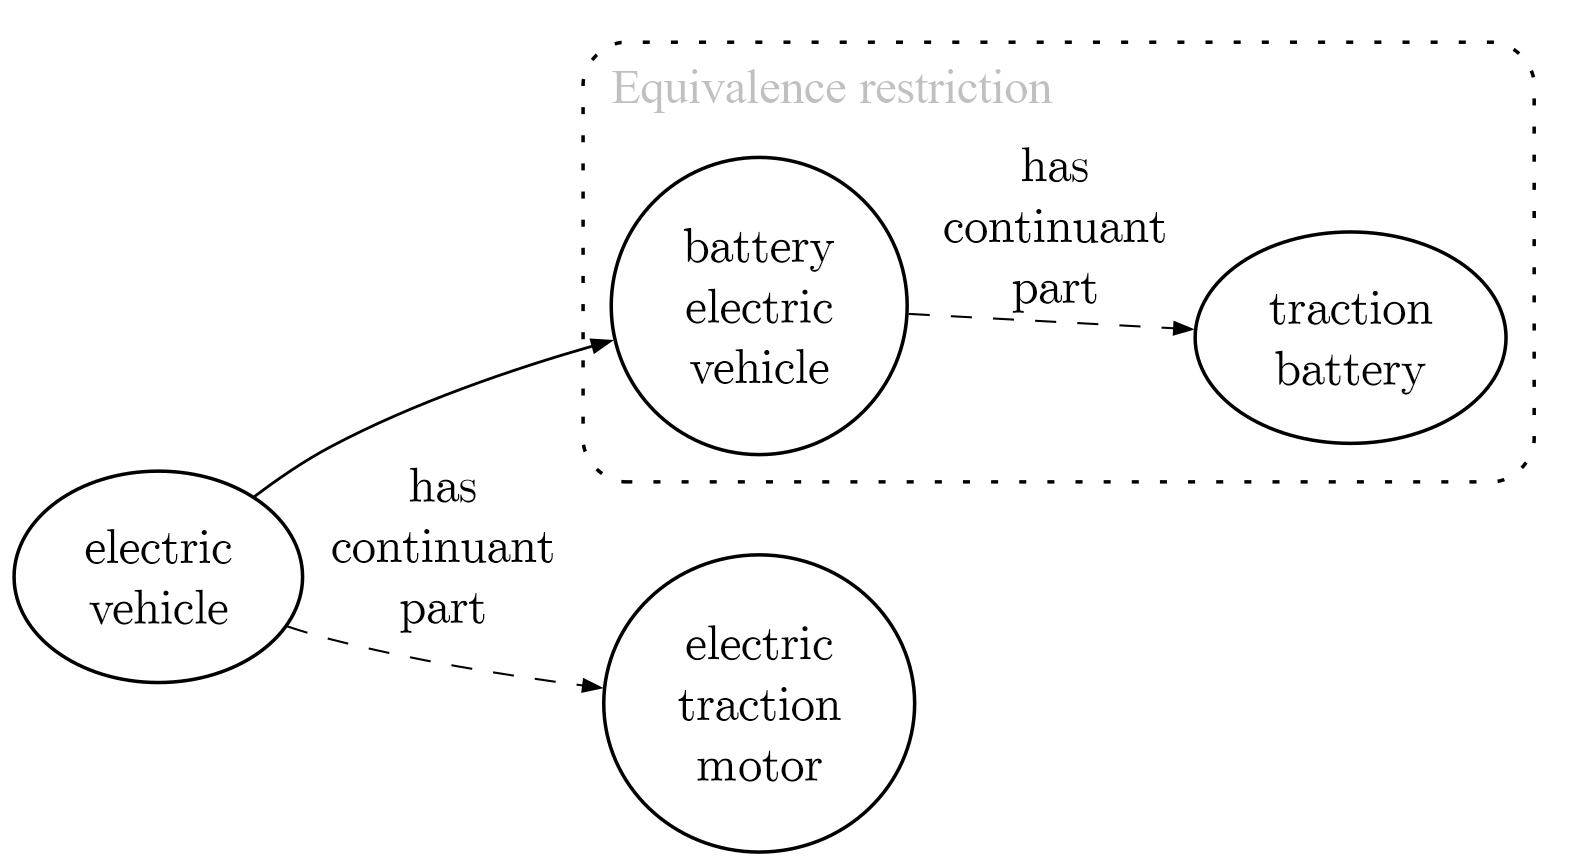
\includegraphics[width=0.9\textwidth]{images/OEOEV}
\end{figure}

\begin{figure}[h]
    \caption{Open energy ontology electric vehicle taxonomy.}
    \centering
    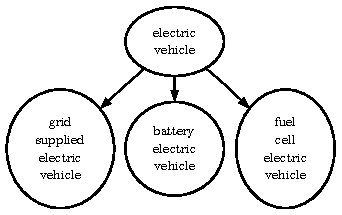
\includegraphics[width=0.6\textwidth]{images/OEOVehicles}
\end{figure}

\subsection{The Common Core Ontologies}

CCO section keywords: Infrastructure, Facilities Vehicle taxonomy

\begin{figure}[h]
    \caption{OEO Vehicle Taxonomy.}
    \centering
    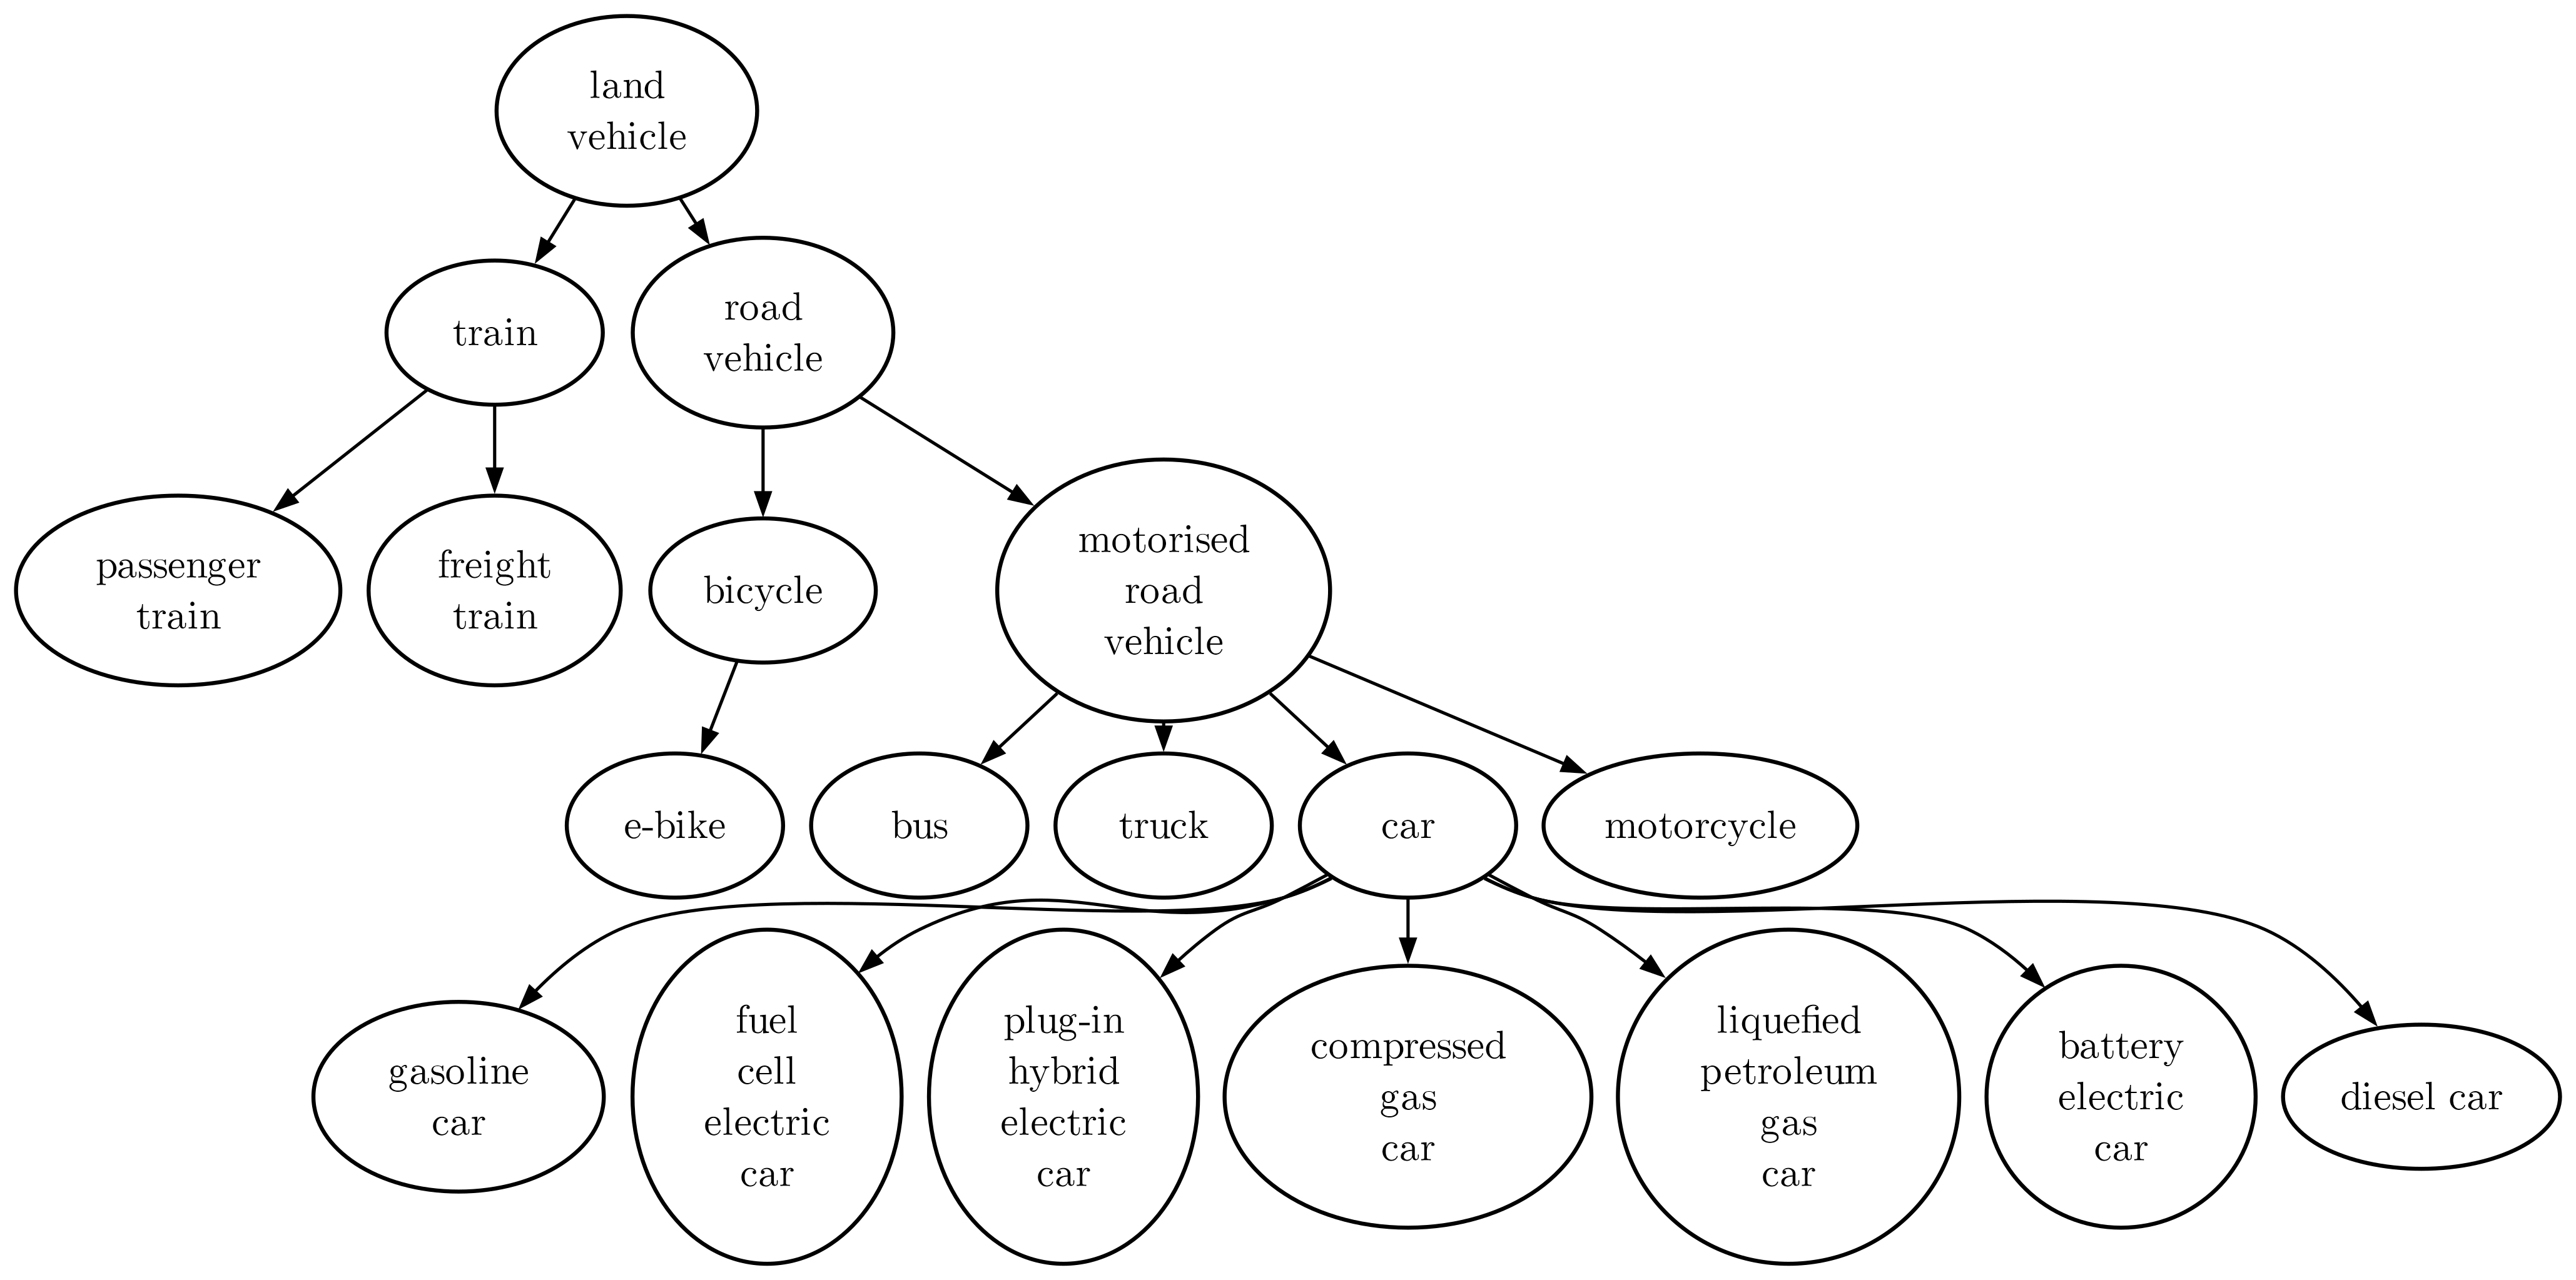
\includegraphics[width=0.9\textwidth]{images/OEOLVehicles}
\end{figure}

\begin{figure}[h]
    \caption{Common Core Ontologies Vehicle Taxonomy.}
    \centering
    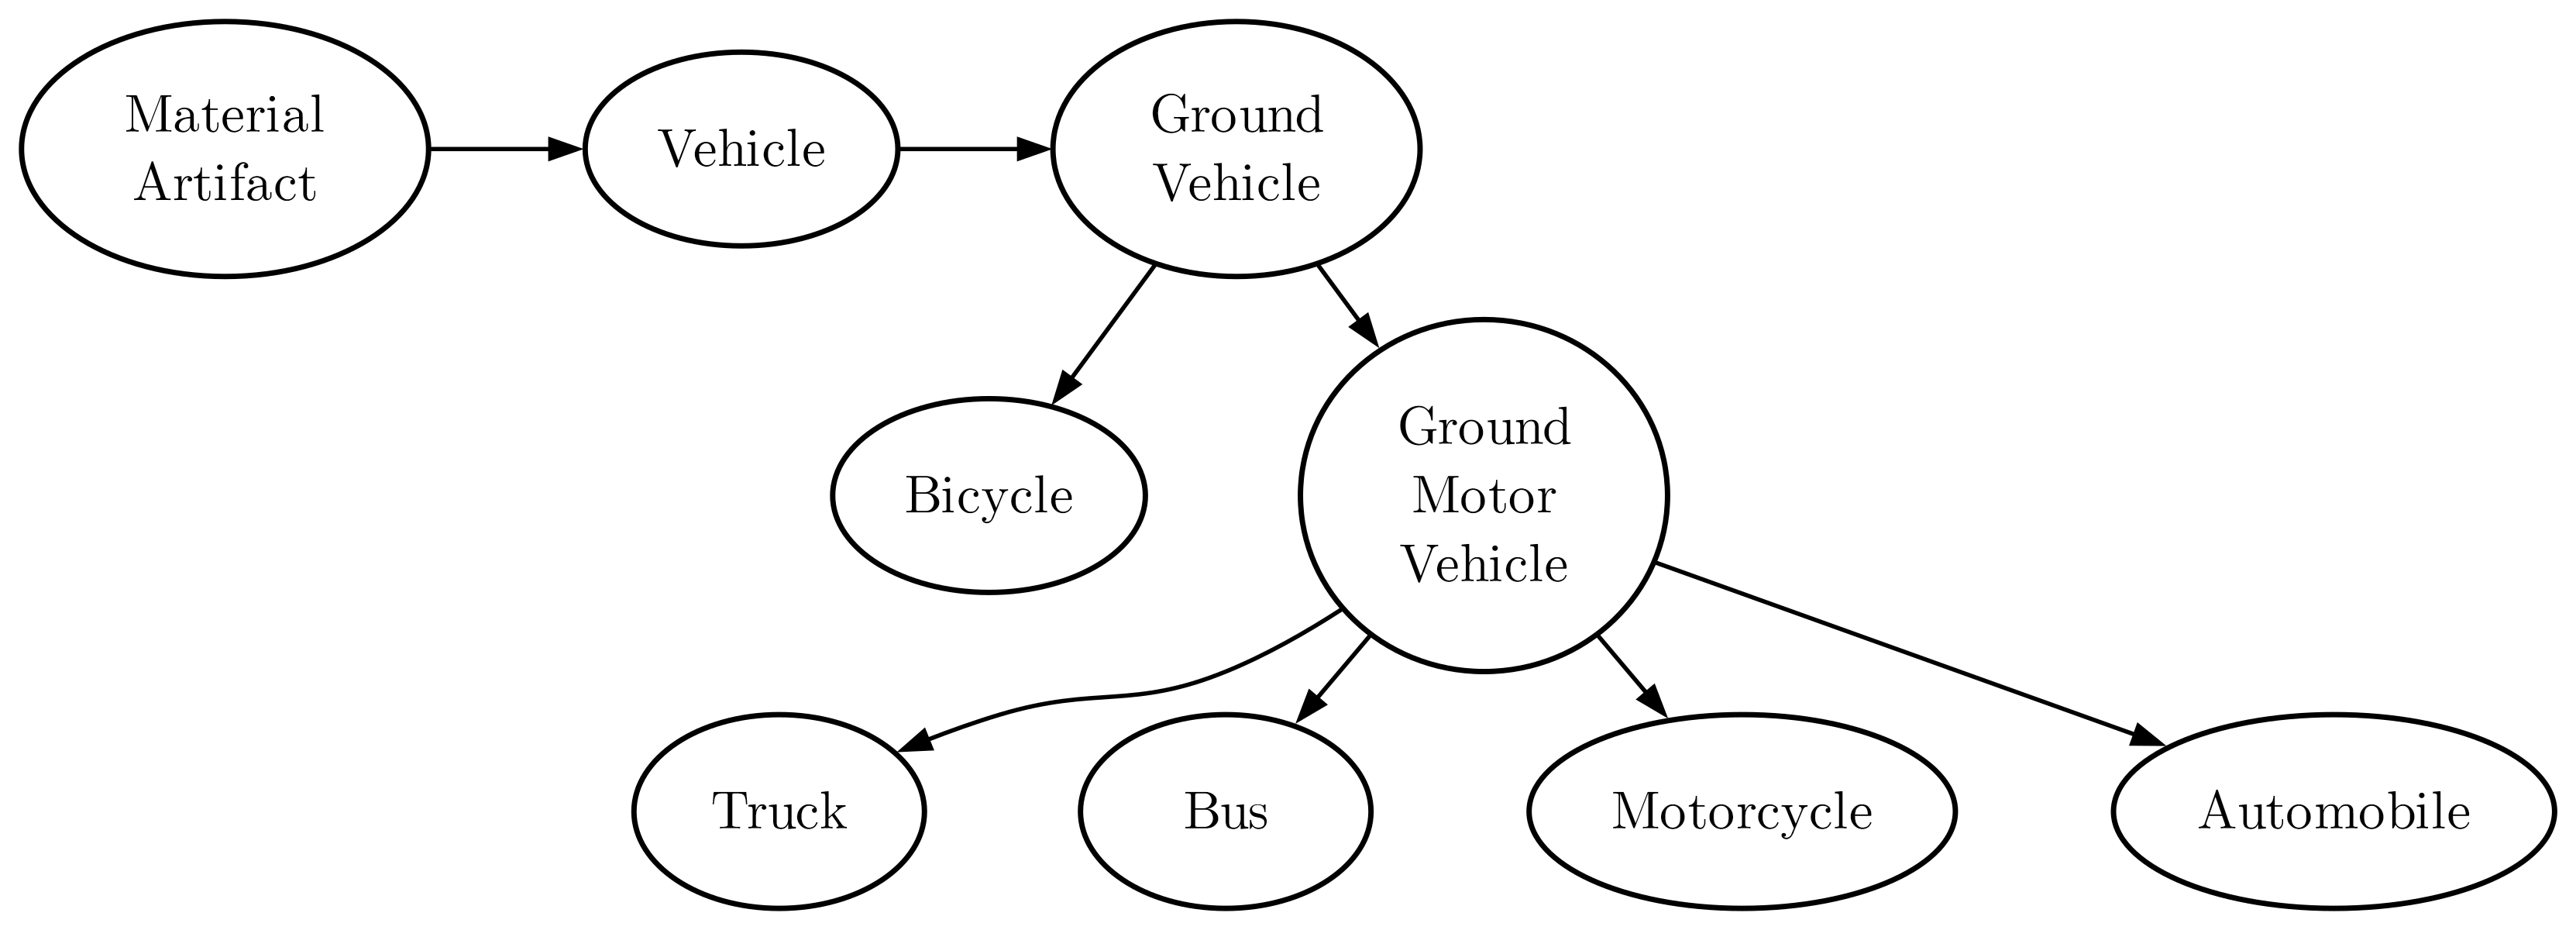
\includegraphics[width=0.9\textwidth]{images/CCOVehicles}
\end{figure}


\begin{figure}[h]
    \caption{Common Core Ontologies infrastructure constraints.}
    \centering
    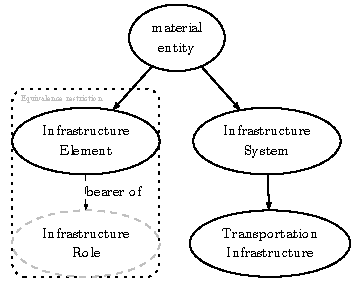
\includegraphics[width=1.0\textwidth]{images/infrastructureSystem}
\end{figure}



\subsection{iCity Parking ontology}

Parking section, keywords: Application specific, different Spatio-temopral assumptions

\begin{figure}[h]
    \caption{iCity parking ontology commitments associated to charging infrastructure.}
    \centering
    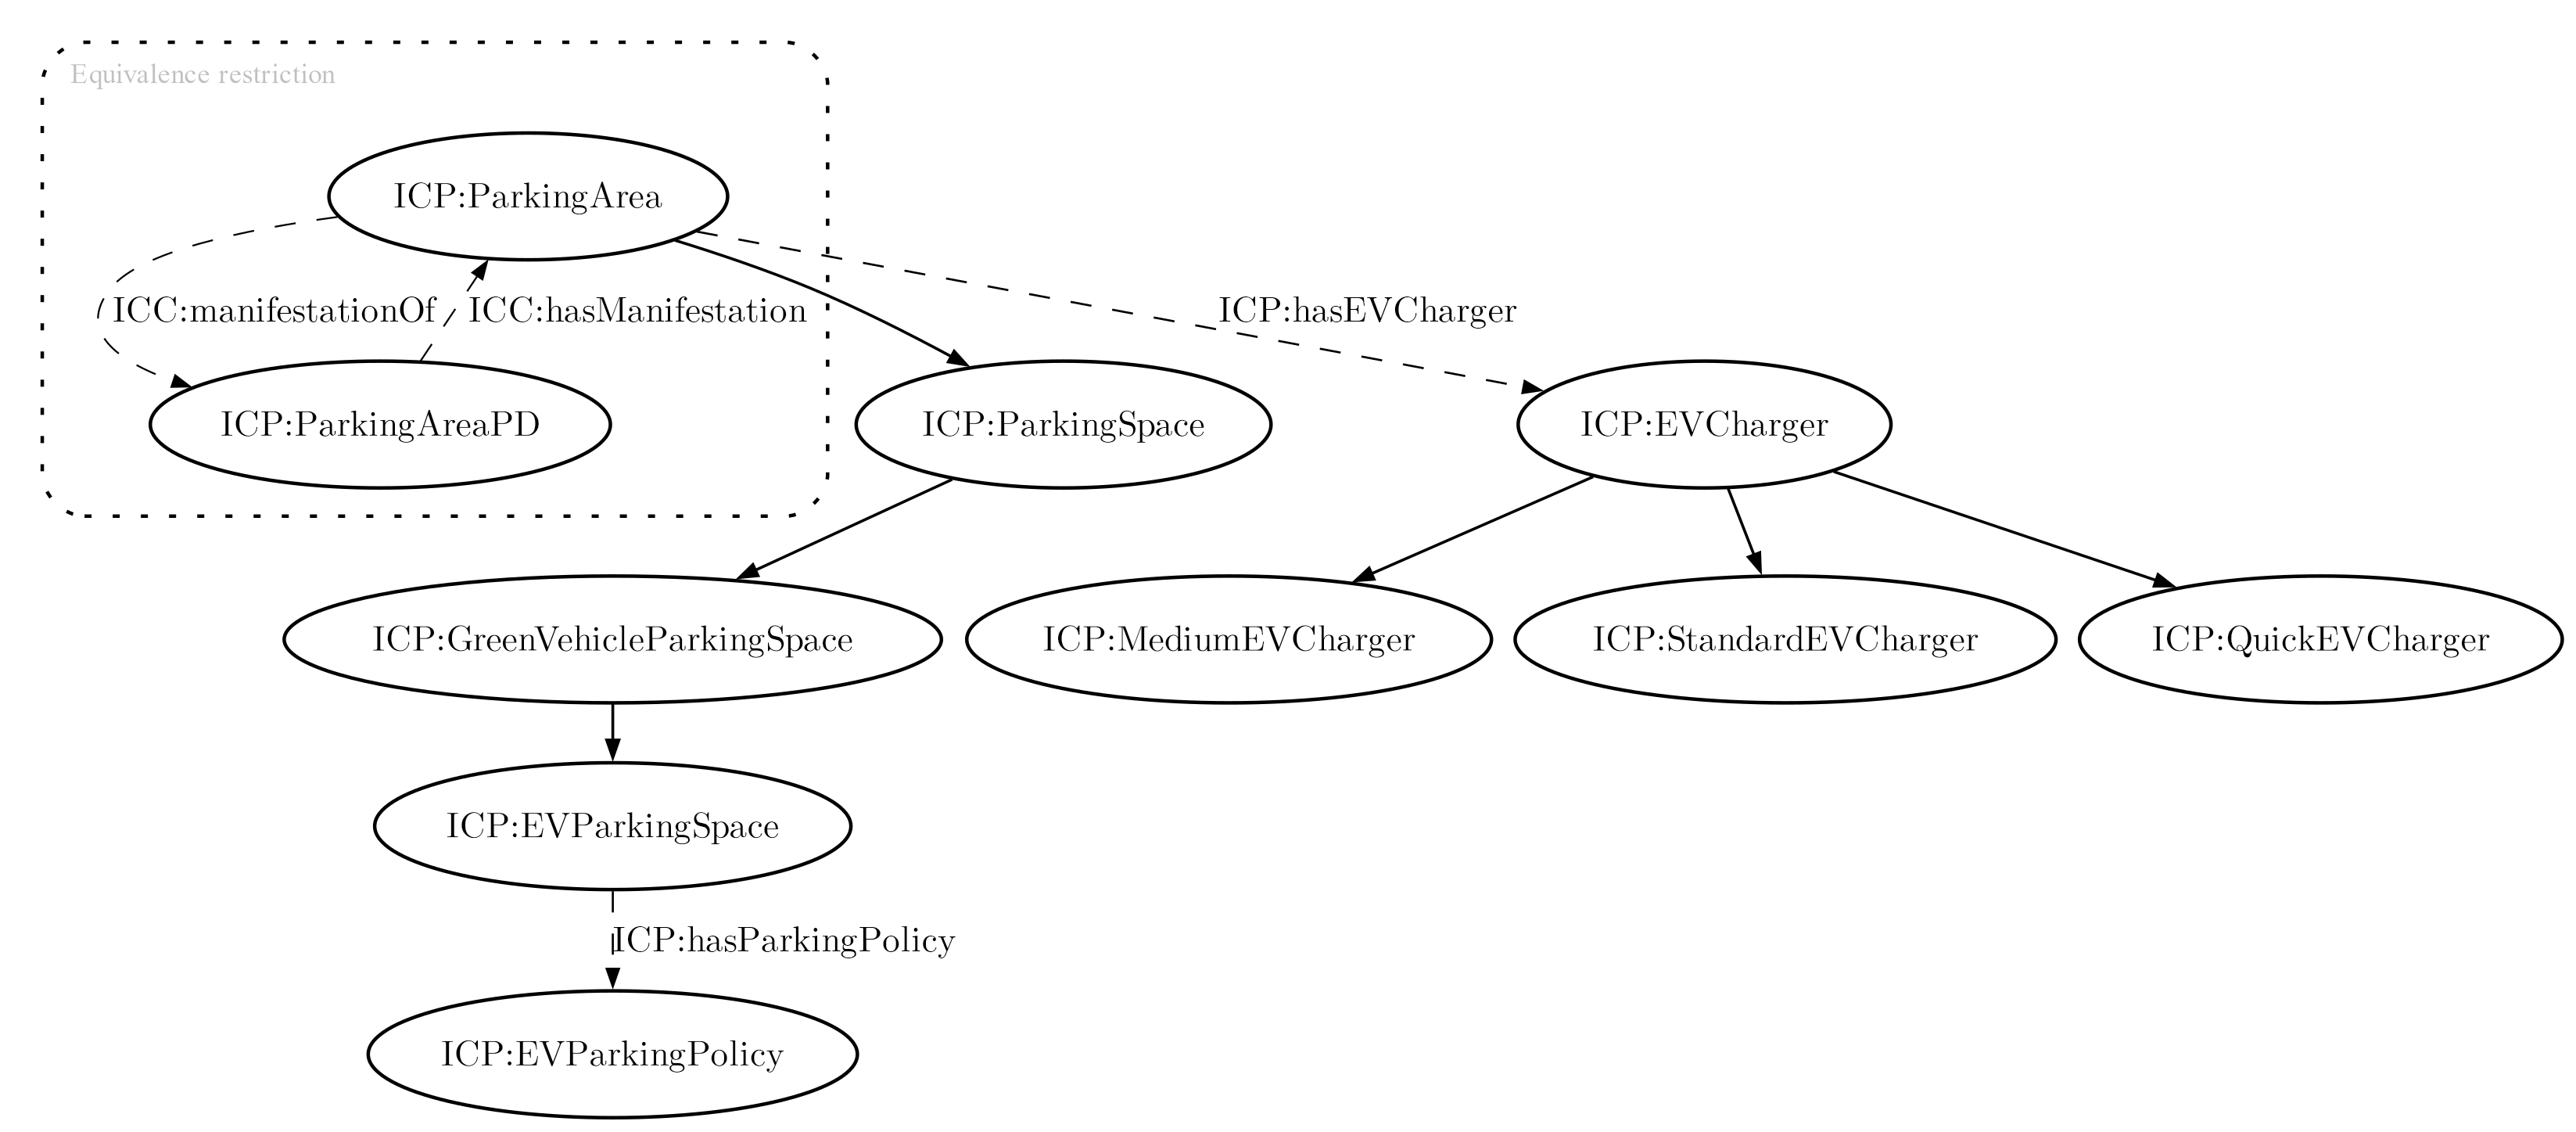
\includegraphics[width=1.0\textwidth]{images/PARKING}
\end{figure}

\subsection{The virtues of using Upper Level Ontologies}
\label{upperlevel}


\subsubsection{The Basic Formal Ontology}

BFO has its own mereology where objects ocupying the same spatiotemporal place
are the same. BFO is bad for materials because it does not consider constitution.
BFO has advantages in regards to object aggreagates, it is relatively easy to represent
membership with it. 
